\documentclass[letter,11pt]{article}

\usepackage[spanish,es-nodecimaldot]{babel}
\usepackage[utf8]{inputenc}

\usepackage{lmodern}
\usepackage[T1]{fontenc}
\usepackage{textcomp}

\usepackage{framed}
\usepackage[svgnames]{xcolor}
\colorlet{shadecolor}{Gainsboro!50}

\usepackage[labelfont=bf]{caption}
\usepackage{graphicx}
\usepackage{pstricks}

\usepackage{anysize}
\marginsize{3cm}{2cm}{2cm}{3cm}

\usepackage{siunitx}
\usepackage{amsmath}
\usepackage{array}
\usepackage{csquotes}
\usepackage{steinmetz}

\usepackage{fancyhdr}
\usepackage{lastpage}
\pagestyle{fancy}
\fancyhf{}
\fancyhead[LE,RO]{Laboratorio de Circuitos Eléctricos III}
\fancyfoot[CO,CE]{\thepage\ de \pageref{LastPage}}

\special{papersize=215.9mm,279.4mm}

\usepackage[
    pdfauthor={Carlos Eduardo Caballero Burgoa},%
    pdftitle={Laboratorio de Circuitos Eléctricos III},%
    pdfsubject={Circuito trifásico fuente estrella y carga estrella equilibrada},%
    colorlinks,%
    citecolor=black,%
    filecolor=black,%
    linkcolor=black,%
    urlcolor=black,
    breaklinks]{hyperref}
\usepackage{breakurl}

\renewcommand{\arraystretch}{1.2}

\begin{document}

\begin{titlepage}
    \begin{center}
        {\Large UNIVERSIDAD MAYOR DE SAN SIMÓN}\\
        \vspace*{0.15cm}
        {\large FACULTAD DE CIENCIAS Y TECNOLOGÍA}\\
        \vspace*{0.10cm}
        DEPARTAMENTO DE ELÉCTRICA-ELECTRÓNICA\\
        \vspace*{3.0cm}
        {\Large \textbf{LABORATORIO DE CIRCUITOS ELÉCTRICOS III}}\\
        \vspace*{0.3cm}
        {\Large \textbf{INFORME No. 1}}\\
        \vspace*{3.5cm}
        {\Large \textbf{CIRCUITO TRIFÁSICO FUENTE ESTRELLA Y \\
        CARGA ESTRELLA EQUILIBRADA}}\\
    \end{center}

    \vspace*{5.8cm}
    \leftskip=7.95cm
    \noindent
    \textbf{Estudiante:}\\
    Caballero Burgoa, Carlos Eduardo.\\
    \newline
    \textbf{Carrera:}\\
    Ing. Electromecánica.\\
    \newline
    \textbf{Docente:}\\
    Ing. Marco Antonio Vallejo Camacho.\\
    \newline
    \textbf{Grupo:} 2F (Martes).\\
\textbf{Fecha de entrega:} 17 de Septiembre del 2024.\\
\end{titlepage}

\section{Cálculos teóricos}
Considerando un circuito trifásico estrella-estrella equilibrado con voltaje de
linea $U_L=380[\text{V}]$ con frecuencia de $50[\text{Hz}]$, se calculan las
corrientes de fase y linea en los siguientes casos:

\vspace{0.6cm}
\subsection{Carga Resistiva}
Se considera una resistencia de $500[\Omega]$.\\

Se calcula el voltaje de fase:
\begin{equation*}
    \begin{split}
        U_F&=\frac{U_L}{\sqrt{3}}\\
           &=\frac{380}{\sqrt{3}}\\
           &=219.39[\text{V}]\\
    \end{split}
\end{equation*}

Para el caso de una resistencia, la impedancia es:
\begin{equation*}
    \begin{split}
        Z&=R\\
         &=500[\Omega]\\
    \end{split}
\end{equation*}

Por tanto, la corriente de linea es:
\begin{equation*}
    \begin{split}
        I_L&=\frac{U_F}{|Z|}\\
           &=\frac{219.39}{500}\\
           &=0.4388[\text{A}]\\
    \end{split}
\end{equation*}

\vspace{0.6cm}
\subsection{Carga Resistiva-Inductiva}
Se considera una resistencia de $500[\Omega]$ y una inductancia de
$0.5[\text{H}]$.\\

Se calcula la frecuencia angular a partir de la frecuencia:
\begin{equation*}
    \begin{split}
        \omega&=2\pi\,f\\
              &=2\pi(50)\\
              &=100\pi[\text{rad}/\text{s}]\\
    \end{split}
\end{equation*}

Para el caso de una resistencia y un inductor, la impedancia es:
\begin{equation*}
    \begin{split}
        Z&=R+j\omega L\\
         &=500+j(100\pi)(0.5)[\Omega]\\
         &=500+j50\pi[\Omega]\\
    \end{split}
\end{equation*}

Por tanto, la corriente de linea es:
\begin{equation*}
    \begin{split}
        I_L&=\frac{U_F}{|Z|}\\
           &=\frac{219.39}{|500+j50\pi)|}\\
           &=\frac{219.39}{\sqrt{500^2+(50\pi)^2}}\\
           &=0.4186[\text{A}]\\
    \end{split}
\end{equation*}

\vspace{0.6cm}
\subsection{Carga Resistiva-Capacitiva}
Se considera una resistencia de $500[\Omega]$ y una capacitancia de
$20[\mu\text{F}]$.\\

Para el caso de una resistencia y un capacitor, la impedancia es:
\begin{equation*}
    \begin{split}
        Z&=R+\frac{1}{j\omega C}\\
         &=R-\frac{j}{\omega C}\\
         &=500-\frac{j}{(100\pi)(\num{20e-6})}[\Omega]\\
         &=500-j\frac{500}{\pi}[\Omega]\\
    \end{split}
\end{equation*}

Por tanto, la corriente de linea es:
\begin{equation*}
    \begin{split}
        I_L&=\frac{U_F}{|Z|}\\
           &=\frac{219.39}{|(500-j\frac{500}{\pi})|}\\
           &=\frac{219.39}{\sqrt{500^2+(500/\pi)^2}}\\
           &=0.4181[\text{A}]\\
    \end{split}
\end{equation*}

\section{Simulación}
Se utilizó el software \emph{Electronic Workbench v5.12.} para simular
los circuitos, estos pueden verse en las figuras: (\ref{simulacion1}),
(\ref{simulacion2}), (\ref{simulacion3}), (\ref{simulacion4}),
(\ref{simulacion5}) y (\ref{simulacion6}).

\begin{figure}[!h]
\centering
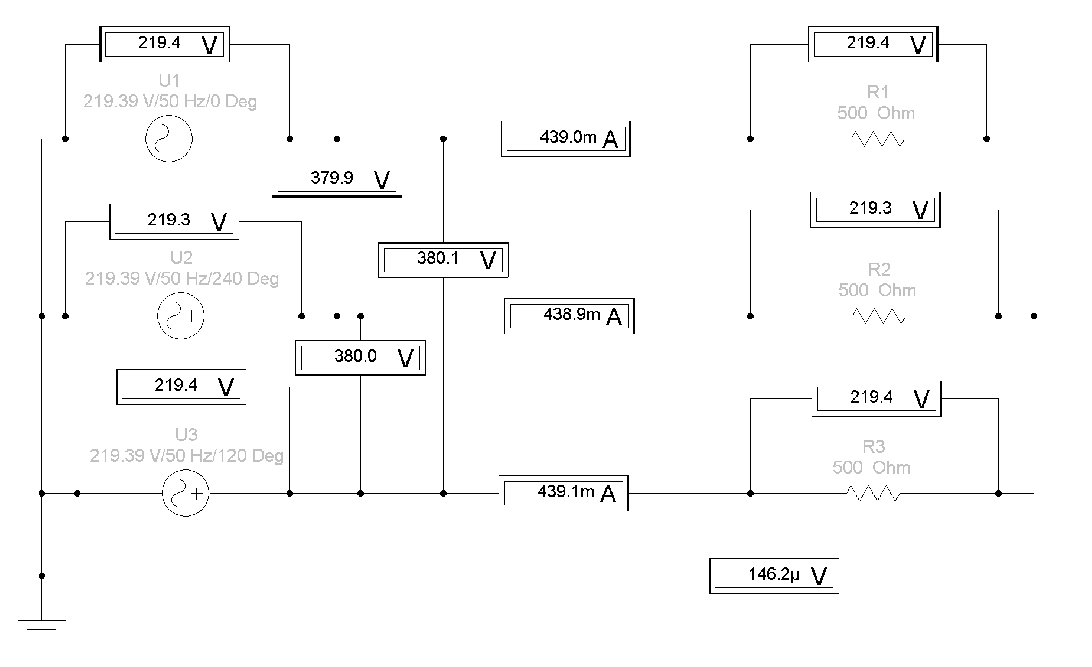
\includegraphics[scale=0.88]{simulacion/practica1.1.eps}
\caption{Simulación del circuito resistivo sin conexión entre neutros.}
\label{simulacion1}
\end{figure}

\begin{figure}[!h]
\centering
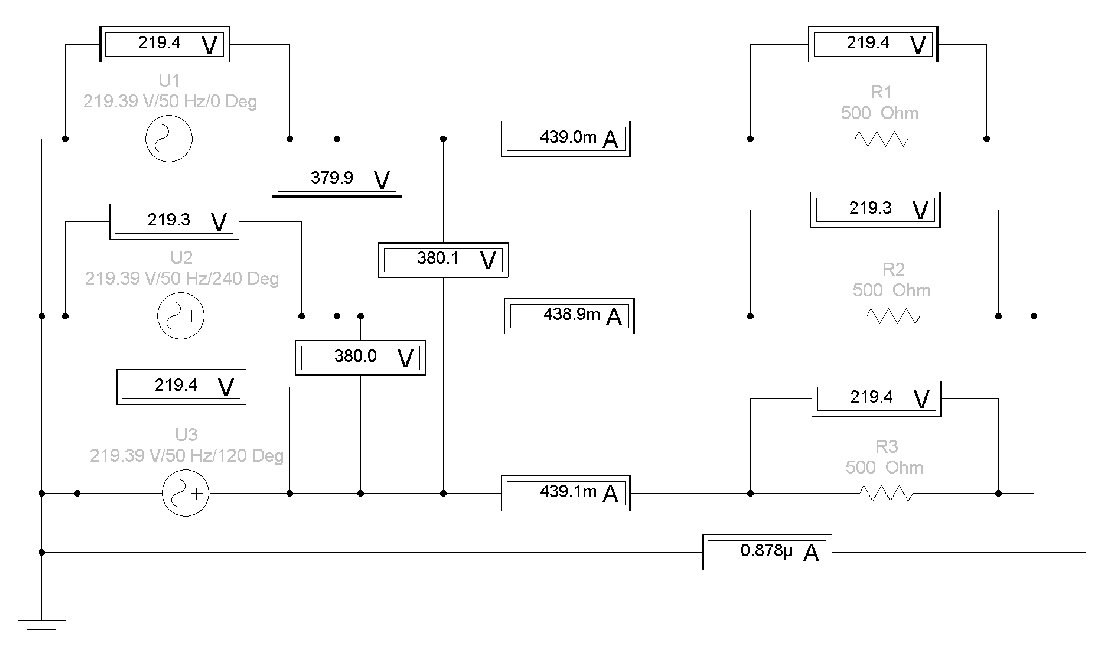
\includegraphics[scale=0.88]{simulacion/practica1.2.eps}
\caption{Simulación del circuito resistivo con conexión entre neutros.}
\label{simulacion2}
\end{figure}

\newpage

\begin{figure}[!h]
\centering
\includegraphics[scale=0.88]{simulacion/practica1.3.eps}
\caption{Simulación del circuito resistivo-inductivo sin conexión entre neutros.}
\label{simulacion3}
\end{figure}

\begin{figure}[!h]
\centering
\includegraphics[scale=0.88]{simulacion/practica1.4.eps}
\caption{Simulación del circuito resistivo-inductivo con conexión entre neutros.}
\label{simulacion4}
\end{figure}

\newpage

\begin{figure}[!h]
\centering
\includegraphics[scale=0.88]{simulacion/practica1.5.eps}
\caption{Simulación del circuito resistivo-capacitivo sin conexión entre neutros.}
\label{simulacion5}
\end{figure}

\begin{figure}[!h]
\centering
\includegraphics[scale=0.88]{simulacion/practica1.6.eps}
\caption{Simulación del circuito resistivo-capacitivo con conexión entre neutros.}
\label{simulacion6}
\end{figure}

\section{Tablas y mediciones}
En las tablas siguientes, se presentan los resultados obtenidos con las
mediciones realizadas en laboratorio.

\subsection{Carga Resistiva}

\begin{center}
    \begin{tabular}{|c||c|c|c||c|c|c||c|c|c|}
    \hline
    & \multicolumn{3}{c||}{\textbf{Voltaje de fase}} & \multicolumn{3}{c||}{\textbf{Voltaje de fase}} & \multicolumn{3}{c|}{\textbf{Voltaje de linea}}
    \tabularnewline
    & \multicolumn{3}{c||}{\textbf{(Generador)}} & \multicolumn{3}{c||}{\textbf{(Carga)}} & \multicolumn{3}{c|}{}
    \tabularnewline \hline
    & $U_{L_1-N}$ & $U_{L_2-N}$ & $U_{L_3-N}$ & $U_{Z_1}$ & $U_{Z_2}$ & $U_{Z_3}$ & $U_{L_1-L_2}$ & $U_{L_2-L_3}$ & $U_{L_3-L_1}$
    \tabularnewline \hline \hline
    \textbf{SN} & $200[V]$ & $223[V]$ & $224[V]$ & $221[V]$ & $224[V]$ & $223[V]$ & $388[V]$ & $392[V]$ & $390[V]$
    \tabularnewline \hline
    \textbf{CN} & $222[V]$ & $224[V]$ & $226[V]$ & $222[V]$ & $225[V]$ & $226[V]$ & $392[V]$ & $395[V]$ & $392[V]$
    \tabularnewline \hline
    \end{tabular}
\end{center}

\begin{center}
    \begin{tabular}{|c||c|c|c||c|c|}
    \hline
    & $I_{L_1}$ & $I_{L_2}$ & $I_{L_3}$ & $I_0$ & $U_0$
    \tabularnewline \hline \hline
    \textbf{SN} & $0.42[A]$ & $0.41[A]$ & $0.44[A]$ & $-$ & $1.30[V]$
    \tabularnewline \hline
    \textbf{CN} & $0.42[A]$ & $0.42[A]$ & $0.45[A]$ & $8.1[mA]$ & $-$
    \tabularnewline \hline
    \end{tabular}
\end{center}

\subsection{Carga Resistiva-Inductiva}

\begin{center}
    \begin{tabular}{|c||c|c|c||c|c|c||c|c|c|}
    \hline
    & \multicolumn{3}{c||}{\textbf{Voltaje de fase}} & \multicolumn{3}{c||}{\textbf{Voltaje de fase}} & \multicolumn{3}{c|}{\textbf{Voltaje de linea}}
    \tabularnewline
    & \multicolumn{3}{c||}{\textbf{(Generador)}} & \multicolumn{3}{c||}{\textbf{(Carga)}} & \multicolumn{3}{c|}{}
    \tabularnewline \hline
    & $U_{L_1-N}$ & $U_{L_2-N}$ & $U_{L_3-N}$ & $U_{Z_1}$ & $U_{Z_2}$ & $U_{Z_3}$ & $U_{L_1-L_2}$ & $U_{L_2-L_3}$ & $U_{L_3-L_1}$
    \tabularnewline \hline \hline
    \textbf{SN} & $221[V]$ & $225[V]$ & $225[V]$ & $223[V]$ & $226[V]$ & $225[V]$ & $392[V]$ & $395[V]$ & $392[V]$
    \tabularnewline \hline
    \textbf{CN} & $223[V]$ & $225[V]$ & $226[V]$ & $223[V]$ & $226[V]$ & $226[V]$ & $392[V]$ & $396[V]$ & $392[V]$
    \tabularnewline \hline
    \end{tabular}
\end{center}

\begin{center}
    \begin{tabular}{|c||c|c|c||c|c|}
    \hline
    & $I_{L_1}$ & $I_{L_2}$ & $I_{L_3}$ & $I_0$ & $U_0$
    \tabularnewline \hline \hline
    \textbf{SN} & $0.40[A]$ & $0.40[A]$ & $0.42[A]$ & $-$ & $2.38[V]$
    \tabularnewline \hline
    \textbf{CN} & $0.39[A]$ & $0.40[A]$ & $0.42[A]$ & $8.9[mA]$ & $-$
    \tabularnewline \hline
    \end{tabular}
\end{center}

\subsection{Carga Resistiva-Capacitiva}

\begin{center}
    \begin{tabular}{|c||c|c|c||c|c|c||c|c|c|}
    \hline
    & \multicolumn{3}{c||}{\textbf{Voltaje de fase}} & \multicolumn{3}{c||}{\textbf{Voltaje de fase}} & \multicolumn{3}{c|}{\textbf{Voltaje de linea}}
    \tabularnewline
    & \multicolumn{3}{c||}{\textbf{(Generador)}} & \multicolumn{3}{c||}{\textbf{(Carga)}} & \multicolumn{3}{c|}{}
    \tabularnewline \hline
    & $U_{L_1-N}$ & $U_{L_2-N}$ & $U_{L_3-N}$ & $U_{Z_1}$ & $U_{Z_2}$ & $U_{Z_3}$ & $U_{L_1-L_2}$ & $U_{L_2-L_3}$ & $U_{L_3-L_1}$
    \tabularnewline \hline \hline
    \textbf{SN} & $223[V]$ & $225[V]$ & $226[V]$ & $224[V]$ & $227[V]$ & $226[V]$ & $393[V]$ & $396[V]$ & $393[V]$
    \tabularnewline \hline
    \textbf{CN} & $223[V]$ & $226[V]$ & $227[V]$ & $223[V]$ & $226[V]$ & $226[V]$ & $393[V]$ & $395[V]$ & $394[V]$
    \tabularnewline \hline
    \end{tabular}
\end{center}

\begin{center}
    \begin{tabular}{|c||c|c|c||c|c|}
    \hline
    & $I_{L_1}$ & $I_{L_2}$ & $I_{L_3}$ & $I_0$ & $U_0$
    \tabularnewline \hline \hline
    \textbf{SN} & $0.41[A]$ & $0.41[A]$ & $0.43[A]$ & $-$ & $1.21[V]$
    \tabularnewline \hline
    \textbf{CN} & $0.41[A]$ & $0.40[A]$ & $0.43[A]$ & $6.7[mA]$ & $-$
    \tabularnewline \hline
    \end{tabular}
\end{center}

\section{Cuestionario}

\begin{enumerate}

\item \textbf{Con los datos de laboratorio el generador es perfectamente
equilibrado?. ¿A qué se debería que no sea así?.}

Los valores difieren levemente, considerando que la variación máxima es de
$4[\text{V}]$ para una medición de $220[\text{V}]$ o superior, se puede
considerar un error despreciable; debido a los instrumentos de medición o el
mismo proceso de medida.

\item \textbf{Determine las relaciones entre tensiones de linea y fase. Se
verifica lo estudiado en la teoría?.}

Considerando los siguientes datos obtenidos:
\begin{center}
    \begin{tabular}{|c||c|c||c|}
    \hline
    & \textbf{Voltaje de fase} & \textbf{Voltaje de linea} & \textbf{Relación $L/F$}
    \tabularnewline \hline \hline
    \textbf{Teórico} & $219.39[V]$ & $380[V]$ & $1.732$
    \tabularnewline \hline
    \textbf{Simulado (promedio)} & $219.39[V]$ & $379.99[V]$ & $1.732$
    \tabularnewline \hline
    \textbf{Laboratorio (promedio)} & $224.11[V]$ & $392.89[V]$ & $1.753$
    \tabularnewline \hline
    \end{tabular}
\end{center}

La relación teórica de $\sqrt{3} (1.7321)$ varia ligeramente en las mediciones
de laboratorio con respecto a la teoría y a la simulación; nuevamente son
cantidades despreciables de error.

\item \textbf{Existe variación en las tensiones de linea y de fase al variar la
carga?. Coincide esto con lo teórico?.}

Considerando los siguientes datos obtenidos:
\begin{center}
    \begin{tabular}{|c||c|c|}
    \hline
    \textbf{Carga} & \textbf{Voltaje de fase} & \textbf{Voltaje de linea}
    \tabularnewline
    & \textbf{(Promedio)} & \textbf{(Promedio)}
    \tabularnewline \hline \hline
    \textbf{Resistivo} & $223.17[V]$ & $391.5[V]$
    \tabularnewline \hline
    \textbf{Resistivo-inductivo} & $224.17[V]$ & $393.17[V]$
    \tabularnewline \hline
    \textbf{Resistivo-capacitivo} & $225[V]$ & $393.83[V]$
    \tabularnewline \hline
    \end{tabular}
\end{center}

Existe una variación de voltaje entre diferentes cargas, aunque en la teoría no
debería existir tal variación, esto variación puede deberse a la variación en la
cantidad de corriente de linea para cada carga, o a problemas relacionados a la
medición.

\item \textbf{El voltaje de neutro medido en cada caso resulta exactamente
cero?. En caso de que no sea así, a que se debe?.}

El voltaje de neutro para cada caso, se resume en la siguiente tabla:
\begin{center}
    \begin{tabular}{|c||c|c||}
    \hline
    & \textbf{Voltaje de neutro}
    \tabularnewline \hline \hline
    Carga resistiva & $1.30[V]$
    \tabularnewline \hline
    Carga resistiva-inductiva & $2.38[V]$
    \tabularnewline \hline
    Carga resistiva-capacitiva & $1.21[V]$
    \tabularnewline \hline
    \end{tabular}
\end{center}

En ningún caso el valor medido fue cero, siendo un voltaje bajo, se puede asumir
que la causa es un ligero desbalance entre las cargas conectadas.

\item \textbf{La corriente de neutro es exactamente cero?. A qué se debe que no
lo sea?.}

La corriente de neutro para cada caso, se resume en la siguiente tabla:
\begin{center}
    \begin{tabular}{|c||c|c||}
    \hline
    & \textbf{Corriente de neutro}
    \tabularnewline \hline \hline
    Carga resistiva & $8.1[mA]$
    \tabularnewline \hline
    Carga resistiva-inductiva & $8.9[mA]$
    \tabularnewline \hline
    Carga resistiva-capacitiva & $6.7[mA]$
    \tabularnewline \hline
    \end{tabular}
\end{center}

En ningún caso el valor medido fue cero, siendo una corriente baja, se puede
asumir que la causa es un ligero desbalance entre las cargas conectadas.

\item \textbf{Existe variación en sus datos obtenidos con neutro físico o sin
neutro físico?. A qué se debería esa variación?.}

Existen pequeñas discrepancias entre las mediciones con neutro y sin neutro
físico, la causa es claramente el mismo desbalance entre las impedancias
conectadas mencionado anteriormente.

\item \textbf{Demostrar mediante diagrama fasorial la relación de voltaje de
linea y de fase:}
\begin{equation*}
    U_L=\sqrt{3}\,U_F
\end{equation*}

El diagrama fasorial puede apreciarse en la figura (\ref{simulacion7}):
\begin{figure}[!h]
\centering
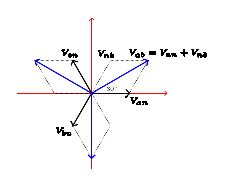
\includegraphics[scale=2.5]{figura1.eps}
\caption{Diagrama fasorial de los voltajes de linea y fase.}
\label{simulacion7}
\end{figure}

Usando la ley de cosenos, y considerando que los voltajes de fase son iguales:
\begin{equation*}
    \begin{split}
        V_{ab}^2&=V_{an}^2+V_{bn}^2-2(V_{an})(V_{bn})\,\cos(180^\circ-30^\circ-30^\circ)\\
                &=V_{an}^2+V_{an}^2-2(V_{an})(V_{an})\,\cos(120^\circ)\\
                &=2V_{an}^2-2\,V_{an}^2\,\cos(120^\circ)\\
                &=2V_{an}^2-2\,V_{an}^2\,(-\frac{1}{2})\\
                &=2V_{an}^2+V_{an}^2\\
                &=3V_{an}^2\\
          V_{ab}&=\sqrt{3}\,V_{an}\\
    \end{split}
\end{equation*}

\end{enumerate}

\section{Conclusiones}
Se demostró experimentalmente la relación entre voltajes de linea y fase para 
un circuito trifásico fuente estrella con carga estrella equilibrada,
comprobándose la relación hallada en la teoría de circuitos eléctricos.

Se calcularon también las corrientes de linea y fase con diferentes impedancias
y también se comprobó que los valores teóricos, simulados, y hallados
experimentalmente no difieren mas allá de lo aceptable.

\end{document}

